\section*{Uvod}

V tej nalogi sem za filtriranje podatkov o GPS koordinatah, hitrostih in pospeških v ravnini uporabljal Kalmanov filter. Ta sestoji iz dveh podkorakov: predict in update ob vsakem času $t_{n+1}$. 

Prvi podkorak uporablja rezultat (kontrolni vektor $\mathbf{x}$) iz prejšnjega časovnega koraka $\mathbf{x}_{n}^+$, kontrolni vektor $\mathbf{c}$ in prehodno matriko sistema $F_n$, ki jo določa izbrani kinematski zakon, s čimer glede na predhodje stanje napove sledeče stanje:
\begin{equation}
    \mathbf{x}_{n+1}^- = F_n\, \mathbf{x}_n^+ + \mathbf{c}
\end{equation}

Drugi podkorak zajema osvežitev stanja z novimi meritvami. Tako dobimo stanje sistema ob času $t_{n+1}$, kjer uporabimo faktor ojačanja $K_{n+1}$, mersko matriko $H_{n+1}$ in vektor meritev $\mathbf{z}_{n+1}$, kar so naši podatki iz datoteke.
\begin{equation}
    \mathbf{x}_{n+1}^+ = \mathbf{x}_{n+1}^- + K_{n+1}\,(\mathbf{z}_{n+1} - H_{n+1}\,\mathbf{x}_{n+1}^-)
\end{equation}

Na podoben način v dveh podkorakih se izvaja tudi izračun kovariančne matrike $P_{n+1}$. Za potrebe filtra je potrebno določiti tudi začetne približke vektorja stanja $\mathbf{x}_0$ in kovariančno matriko $P_0$. Vektorje in matrike sem uporabljal take, kot so v navodilih, prav tako tudi časovni korak $\Delta t$ in napake meritev.

\section*{Testni primer}

Kot prvo sem preizkusil delovanje Kalmanovega filtra v preprostem 1D primeru $(x,v_x)$. Predpostavil sem gibanje s konstantno hitrostjo 1 m/s in podatkom o pomiku dodal naključen beli šum. Te podatke sem nato analiziral s filtrom in ugotovil njega pravilno delovanje. Podatke o pomikih dobimo manj zašumljene, hitrost pa ni več taka, kot bi morala biti. Potrebno pa je opomniti, da hitrost ni bila zajeta v vektorju meritev $\mathbf{z}$.

\begin{figure}[ht!]
    \centering
    \begin{minipage}{0.45\textwidth}
        \centering
        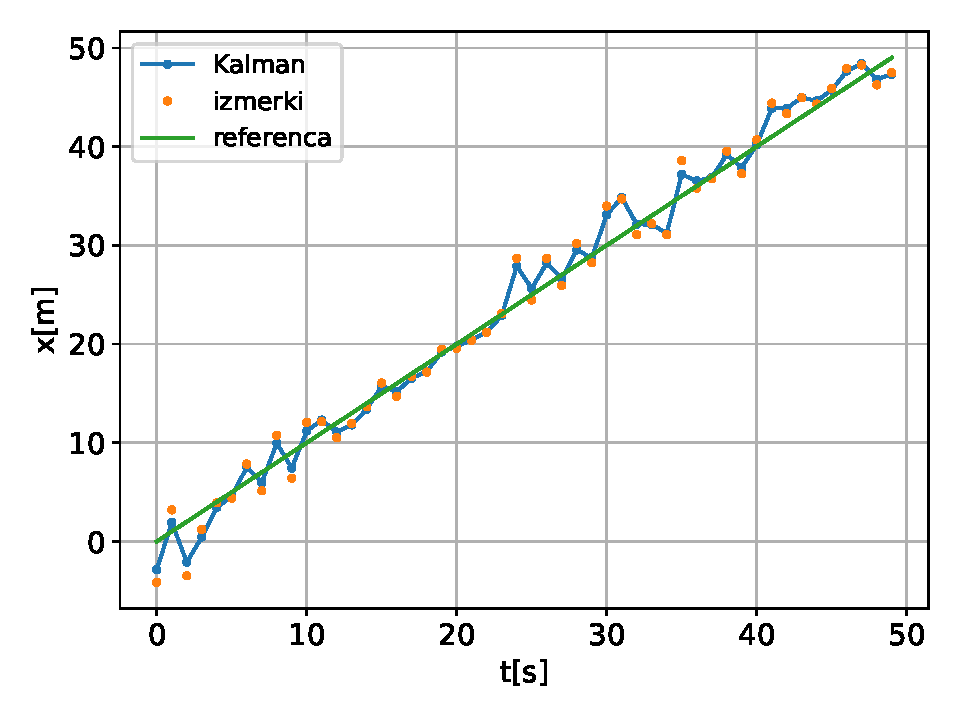
\includegraphics[width=0.9\linewidth]{11.nal_slike/test_1d_x.pdf}
        \caption{Filtrirana pot v 1D}
    \end{minipage}
    \begin{minipage}{0.45\textwidth}
        \centering
        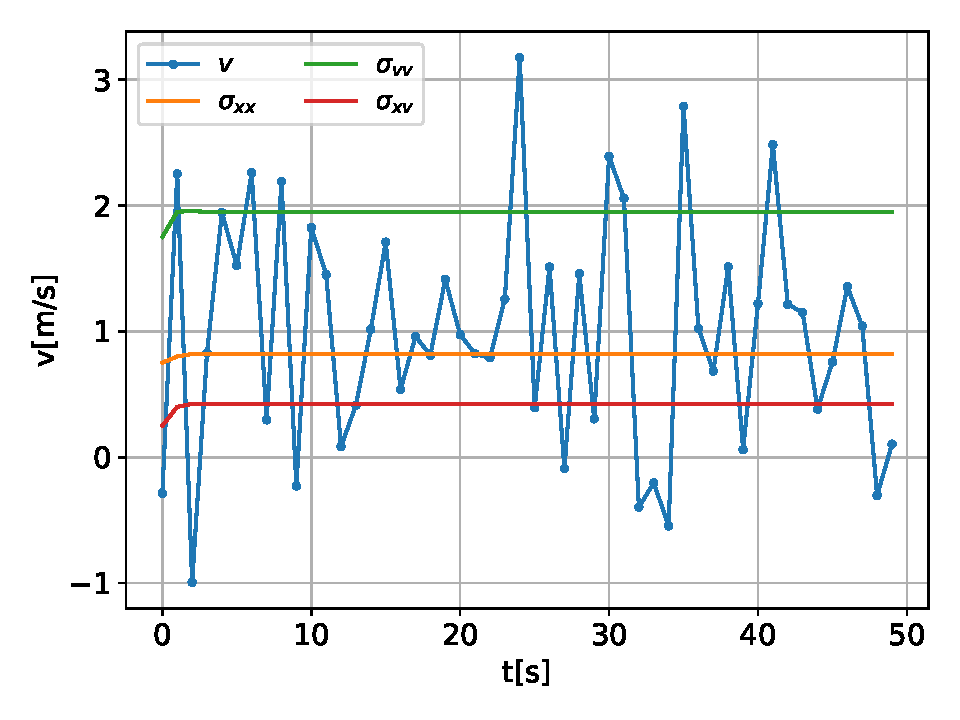
\includegraphics[width=0.9\linewidth]{11.nal_slike/test_1d_v.pdf}
        \caption[short]{Potek napake hitrosti in varianc}
    \end{minipage}
\end{figure}

%%%%%%%%%%%%%%%%%%%%%%%%%%%%%%%%%%%%%%%%%%%%%%%%%%%%%%%%%%%
\section{Filtriranje v Kartezičnem koordinatnem sistemu}

Ravninsko gibanje sem filtriral s Kalmanovim filtrom in pri tem upošteval vsak časovni korak $\Delta t$. Kinematični zakon predpostavlja premo enakomerno gibanje, kot je navedeno v predlogi. Ob primerjavi na sliki je le v detajlu opazno malenkostno odstopanje od referenčne poti, v globalnem napaka ni opazna. Filter lepo sledi izmerkom.

\begin{figure}[ht!]
    \centering
    \begin{minipage}{0.49\textwidth}
        \centering
        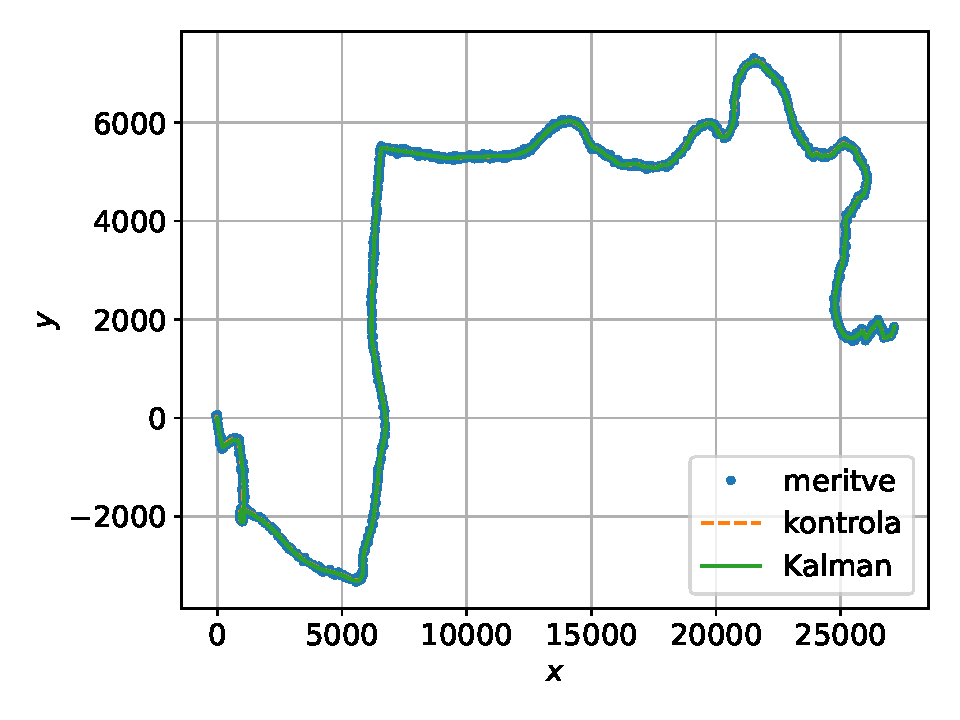
\includegraphics[width=\textwidth]{11.nal_slike/pot_vse.pdf}
        \caption{Celotna pot}
    \end{minipage}
    \begin{minipage}{0.49\textwidth}
        \centering
        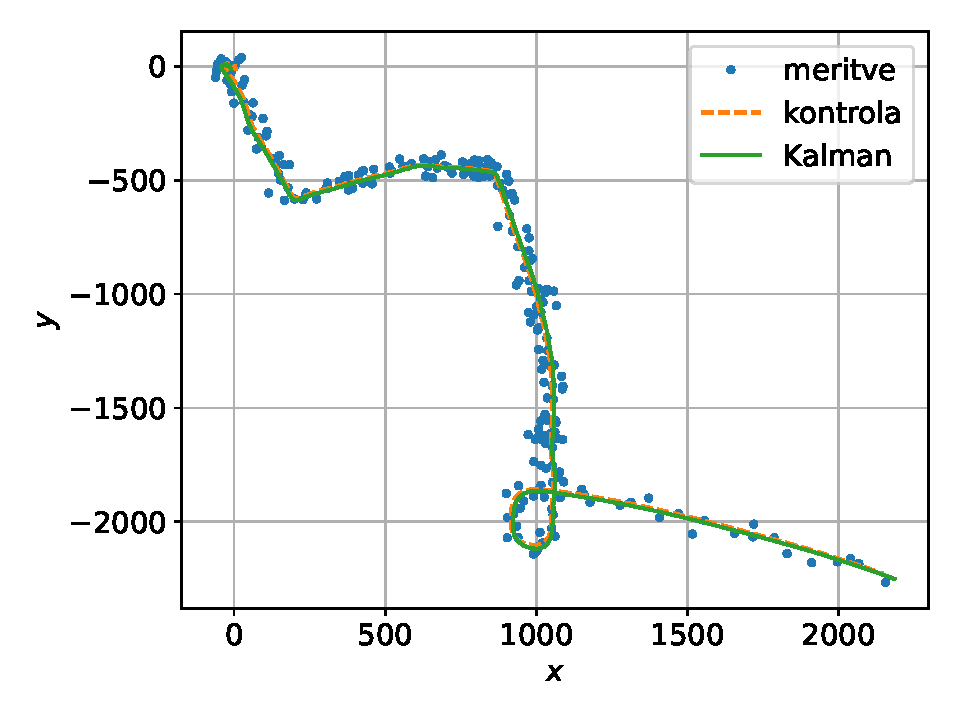
\includegraphics[width=\textwidth]{11.nal_slike/pot_detajl.pdf}
        \caption[short]{Detajl filtrirane poti in primerjava s kontrolo}
    \end{minipage}
\end{figure}

Če izrišem še potek hitrosti, ki so bile v tem primeru zajete pri podkoraku ``update" v vektorju meritev $\mathbf{z}$. Opazimo, da potek hitrosti filtra lepo sledi kontroli, le pri nekaterih ekstremih ima filter večje odmike. Med izmerki in filtrom ni tako očitne razlike, iz tega lahko sklepamo, da na tak način ne moremo pridobiti bolj napančnih informacij iz podatkov ali pa so le-te že dovolj natančne. Zanimvo je tudi, da lahko na tak način, ob pomoči koordinat in zemljevida spremljamo, kako se je voznik držal omejitev. Opazil sem, da je značilne omejitve hitrosti v in izven naselja ter na avtocesti nekajkrat celo presegel!

\begin{figure}[H]
    \centering
    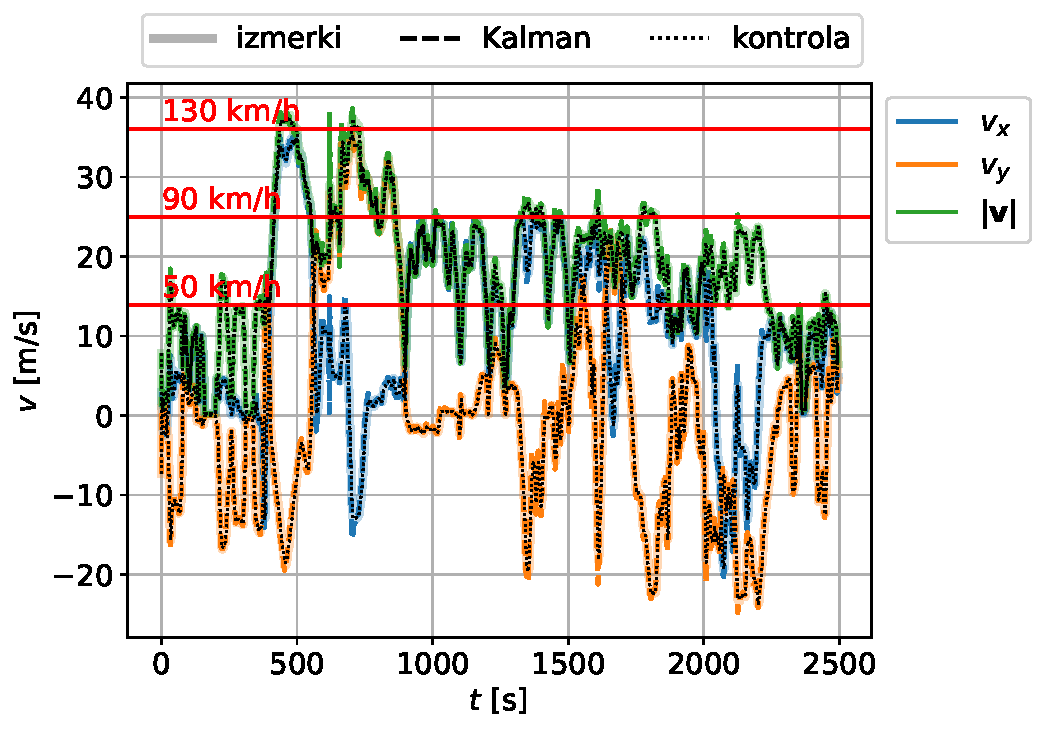
\includegraphics[width=0.6\textwidth]{11.nal_slike/potek_hitrosti.pdf}
    \caption[short]{Potek hitrosti tekom poti}
\end{figure}

Pri analizi odstopanj med rezultati filtra in kontrolo lahko opazimo, da dobimo očitno manj šuma na podatkih lege in malenkost več pri hitrosti. Če podatke zapišemo v brezkoordinatni obliki (skalarno), je še vedno izrazit vrh napake poti pri okoli 500 s, pri hitrosti ta ni opazen. Obratno je pri cca. 600 s, kjer je vrh napake hitrosti, pri legi pa je tam lahko rečem minimum. Ocenjena napaka meritve lege in hitrosti je sicer po filtriranju nekajkrat presežena, vendar v splošnem pod ocenjeno vrednostjo.

\begin{figure}[H]
    \centering
    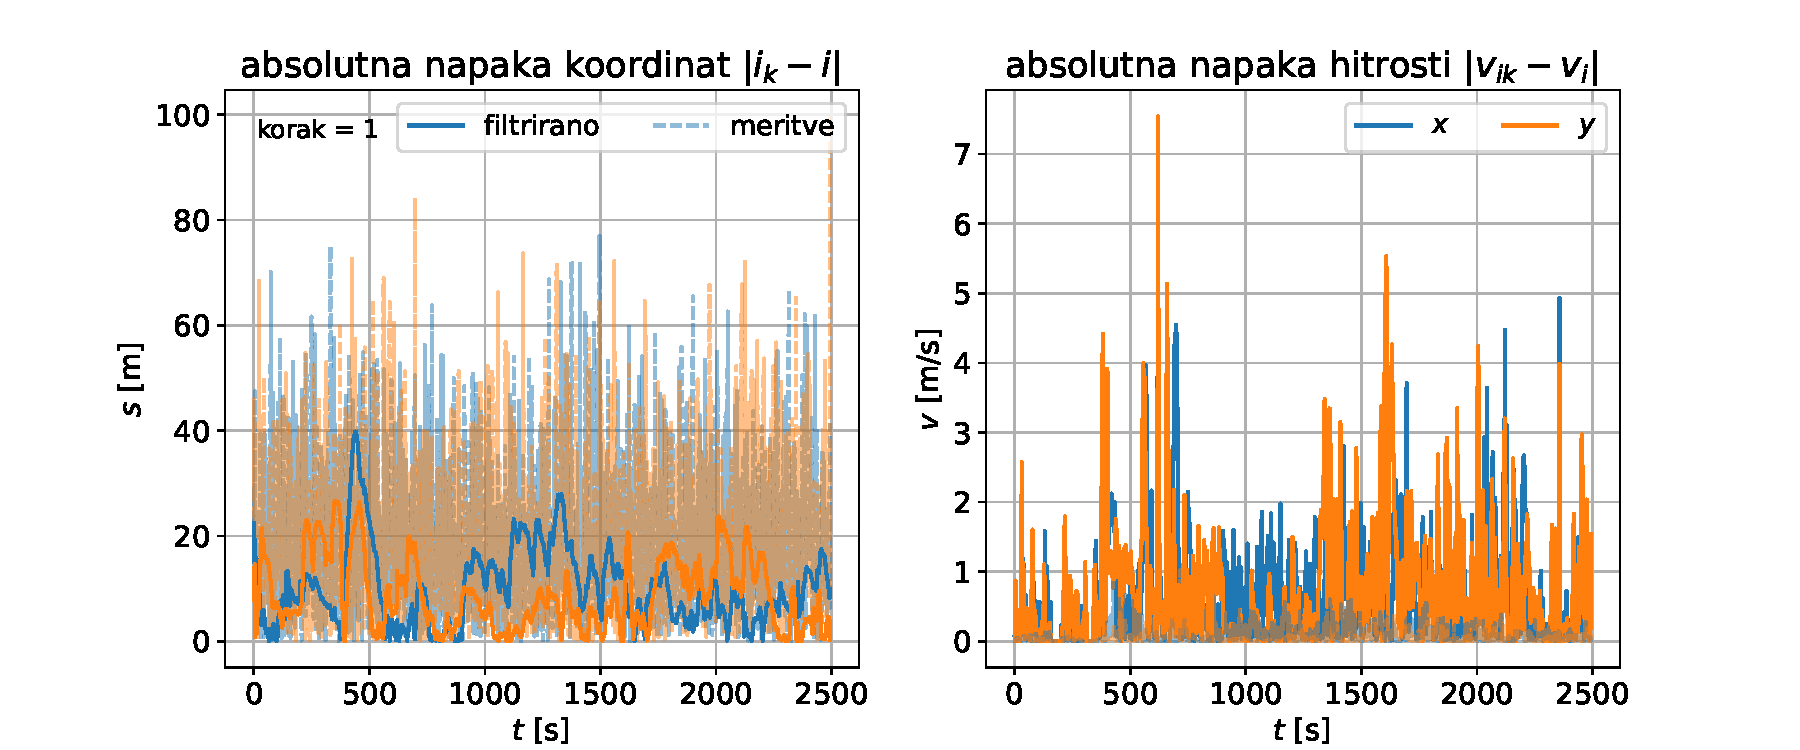
\includegraphics[width=0.9\textwidth]{11.nal_slike/napaka_po_koor.pdf}
    \caption[short]{Potek napak filtriranih vrednosti po koordinatah}
\end{figure}

\begin{figure}[H]
    \centering
    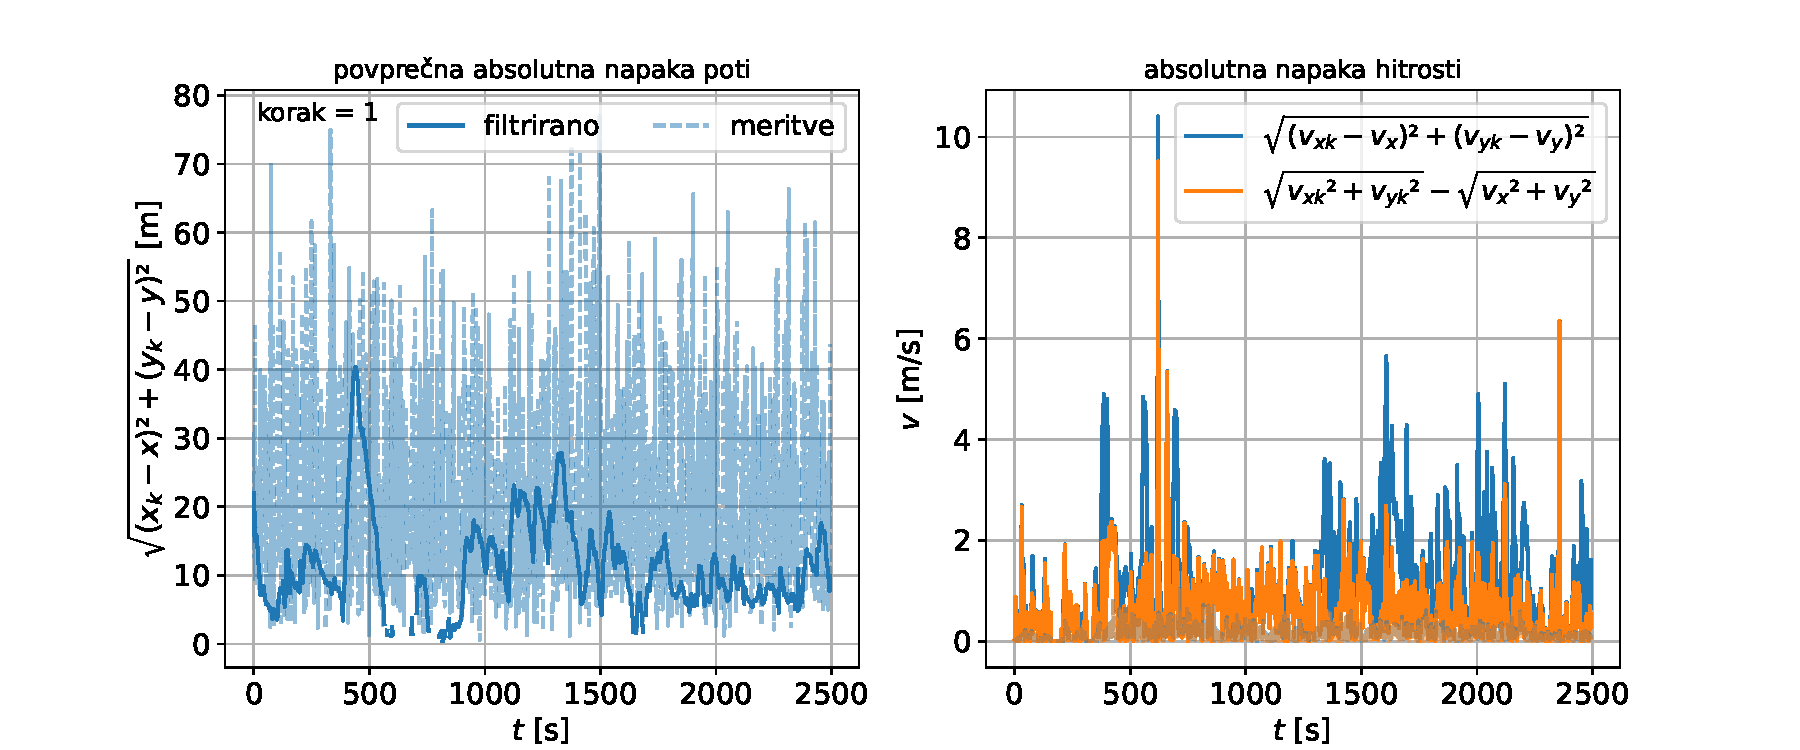
\includegraphics[width=0.9\textwidth]{11.nal_slike/napaka_poti_hitrosti.pdf}
    \caption[short]{Potek napak filtriranih vrednosti brezkoordinatno}\label{fig:napake}
\end{figure}

%%%%%%%%%%%%%%%%%%%%%%%%%%%%%%%%%%%%
    \subsection{Različne frekvence vzorčenja -- koraki}\label{sec:koraki}

Pri podatkih lahko spreminjamo frekvenco vzorčenja tako, da periodično izpuščamo podatke. Periodo tega imenujem ``korak'', če je le-ta enak 1 pomeni, da so upoštevani vsi podatki, pri koraku N pa vsak N-ti podatek/izmerek, vmes pa jih je N-1 izpuščenih. Ta princip lahko uporabimo enakomerno na vseh podatkih v vektorju stanja $\mathbf{x}$ ali pa posebej na vsaki komponenti. Jaz sem uporabljal posebej korak na veličinah lege in hitrosti, od katerih odvisnost prikazuje spodnji graf. To sem storil tako, da sem spreminjal mersko matriko $H$ -- njene diagonalne vrednosti v update podkoraku.\\
Opomba: skupni residual veličine $a(t)$ glede na referenco $a_{ref}(t)$ je izračunan: $|a_i - a_{ref, i}|$

Opazen je trend, da pri večanju skupnega koraka enakomerno (diagonala po grafu), napaka raste. Hkrati pa vidimo, da je napaka veliko bolj občutljiva na korak hitrosti, kot od lege. Zanimivo je tudi, da obstajajo ``otoki'', kjer so lokalni minimumi napake. Iz tega sklepam, da je sistem nelinearen. Vseeno velja poudariti, da je pri večanju koraka napaka že dokaj velika in zato pogosto presega ocenjeno napako meritve in izračunane kovariance iz filtra. V tem primeru bi morali korigirati začetni približek kovariančne matrike in pri tem upoštevati tudi napako zaradi manj meritev.

\begin{figure}[H]
    \centering
    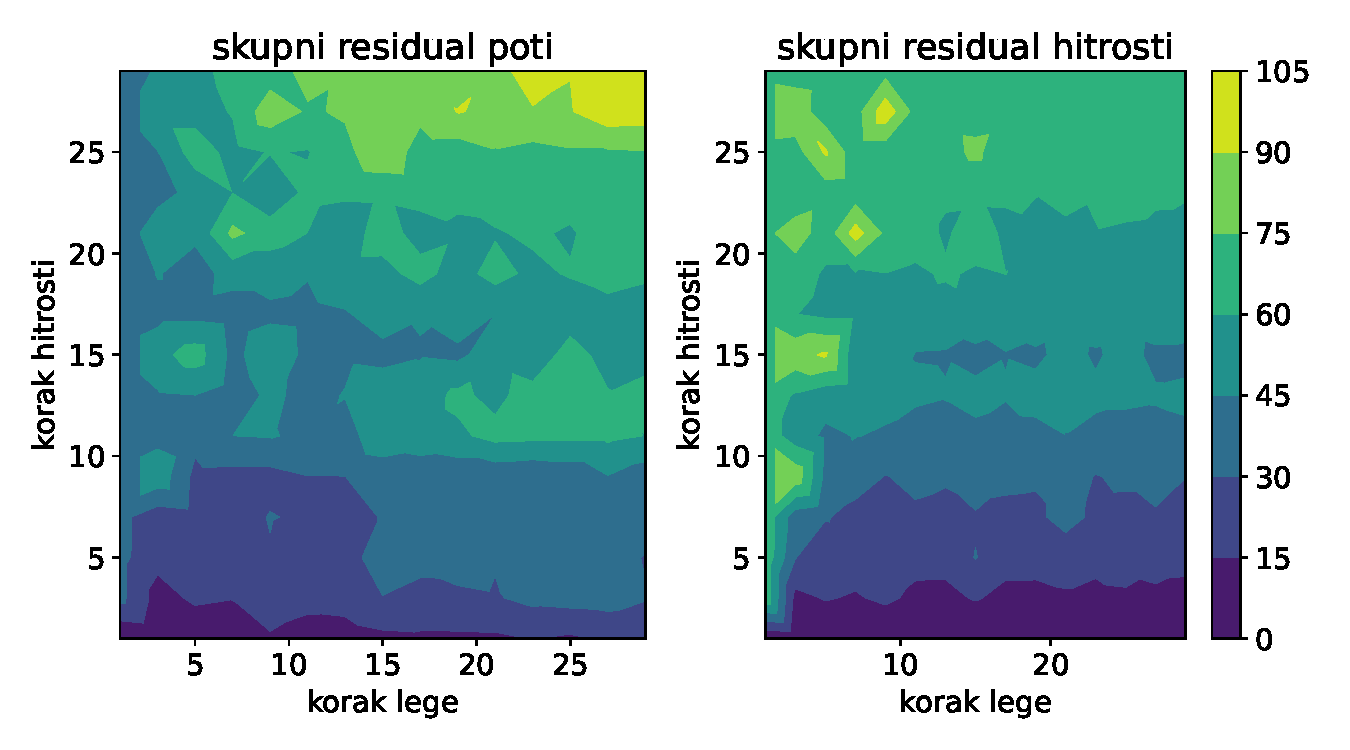
\includegraphics[width=0.8\textwidth]{11.nal_slike/vpliv_korakov_2dplot.pdf}
    \caption[short]{skupni skalirani residual (0-100\%) je odvisen od koraka}   
\end{figure}

    \subsection{Residuali}

Lahko spremljano tudi residuale posebej, kot $f(t, korak)$. Pri tem je uporabljen enak korak hitrosti in poti, residuali pa so izračunani kot $|| \mathbf{k}_n - H\,\mathbf{x}_n ||$, kjer je $\mathbf{k}_n$ vektor referenčnega stanja v $n$-tem koraku. Podobno bi dobili, če bi namesto $\mathbf{k}$ uporabili $\mathbf{z}$, kot je predlagano v navodilih, vendar sem mnenja, da je bolje primerjati s pravilnimi (referenčnimi) rezultati, ako so na voljo.  Pri tem opazimo izrazit padec residuala vsakič, ko osvežimo filter z novimi podatki, kar je posebej opazno pri večjem koraku. Zanimivo je, da se krivulje različnih korakov prekrivajo, za kar je kriva narava filtra.
\begin{figure}[H]
    \centering
    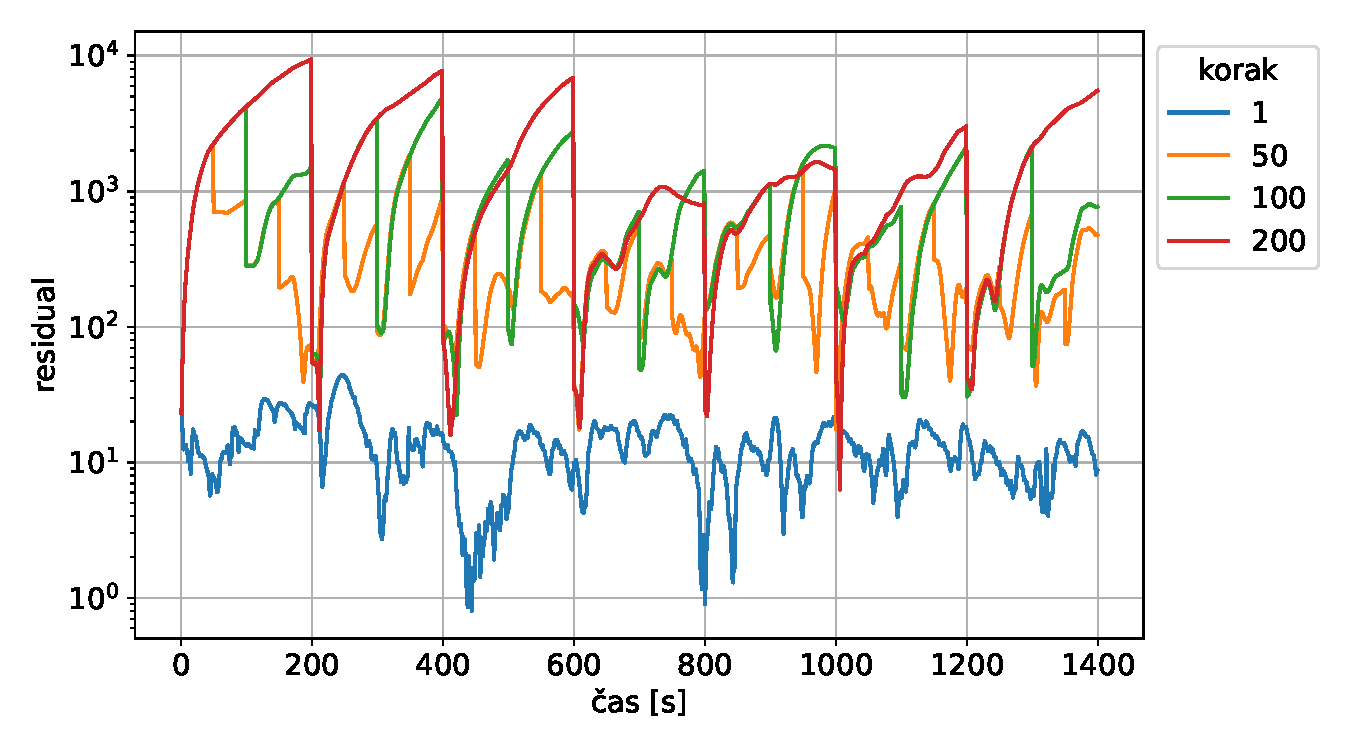
\includegraphics[width=0.75\textwidth]{11.nal_slike/residuali.pdf}
    \caption[short]{Potek residualov pri različnih korakih podatkov}
\end{figure}

\subsection{Kovariance}

Kot je že omenjeno v uvodu, s Kalmanovim filtrom računamo tudi kovariančno matriko $P_n$, čeprav je do seedaj nisem obravnaval pa igra pomembno vlogo pri določitvi faktorja ojačanja $K_{n}$ v vsakem koraku. Kovariančni matriki je posvečeno to poglavje. Sicer nisem bil prepričan, kako naj predstavim matriko, saj bi bil potek za vsako komponento preveč nepregleden na enem grafu (matrika je 4x4!), vendar sem se na koncu odločil, da prikažem determinanto. Ta odraža nekakšno povprečje celotne matrike in kot je prikazano na spodnji sliki, tudi lepo sledi trendu.

Opazno je tudi, da večji korak viša vrednosti determinante, kovariance so v splošnem večje. Takrat so tudi večje oscilacije vrednosti. Trije izraziti minimumi so verjetno posledica singularnosti v matriki in domnevam, da nimajo fizikalnega ozadja.

\begin{figure}[H]
    \centering
    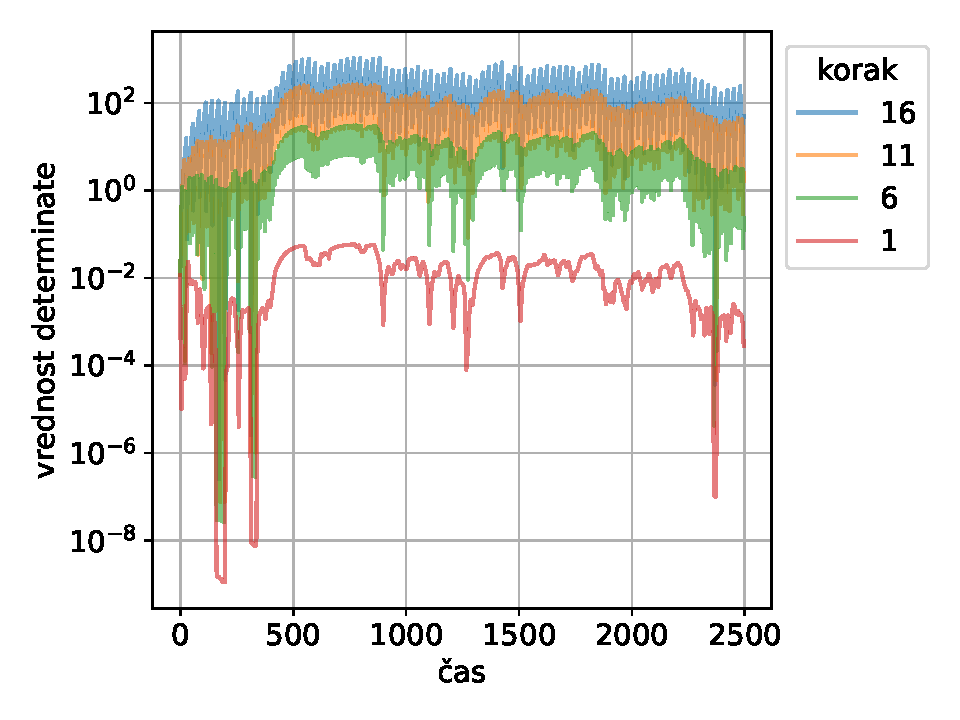
\includegraphics[width=0.6\textwidth]{11.nal_slike/det_cov_matrike.pdf}
    \caption[short]{Potek determinante kovariančne matrike pri različnih korakih podatkov}
\end{figure}

    \subsection{Napačen začetni približek}

Do sedaj sem za začetni približek vektorja stanja vzel prvo meritev, v tem poglavju pa se sprašujem, kako sprememba tega vpliva na rezultat. Na sliki je residual skupen skaliran, kot v poglavju \ref{sec:koraki}. Poizkušal sem zamikati začetno lego za $\pm500$ m in ugotovil zanimive lastnosti: na tak način lahko celo zmanj šamo napako hitrosti! Vendar pa vsak odmik poveča napako lege, a graf ni povsem simetričen. Začetna hitrost je tudi zanimiva: če spremenimo obe komponenti linearno, to ne vpliva na razultat, najslabše pa je, če eno večamo, drugo manjšamo. To vpliva enako na napako poti in hitrosti.

\begin{figure}[H]
    \centering
    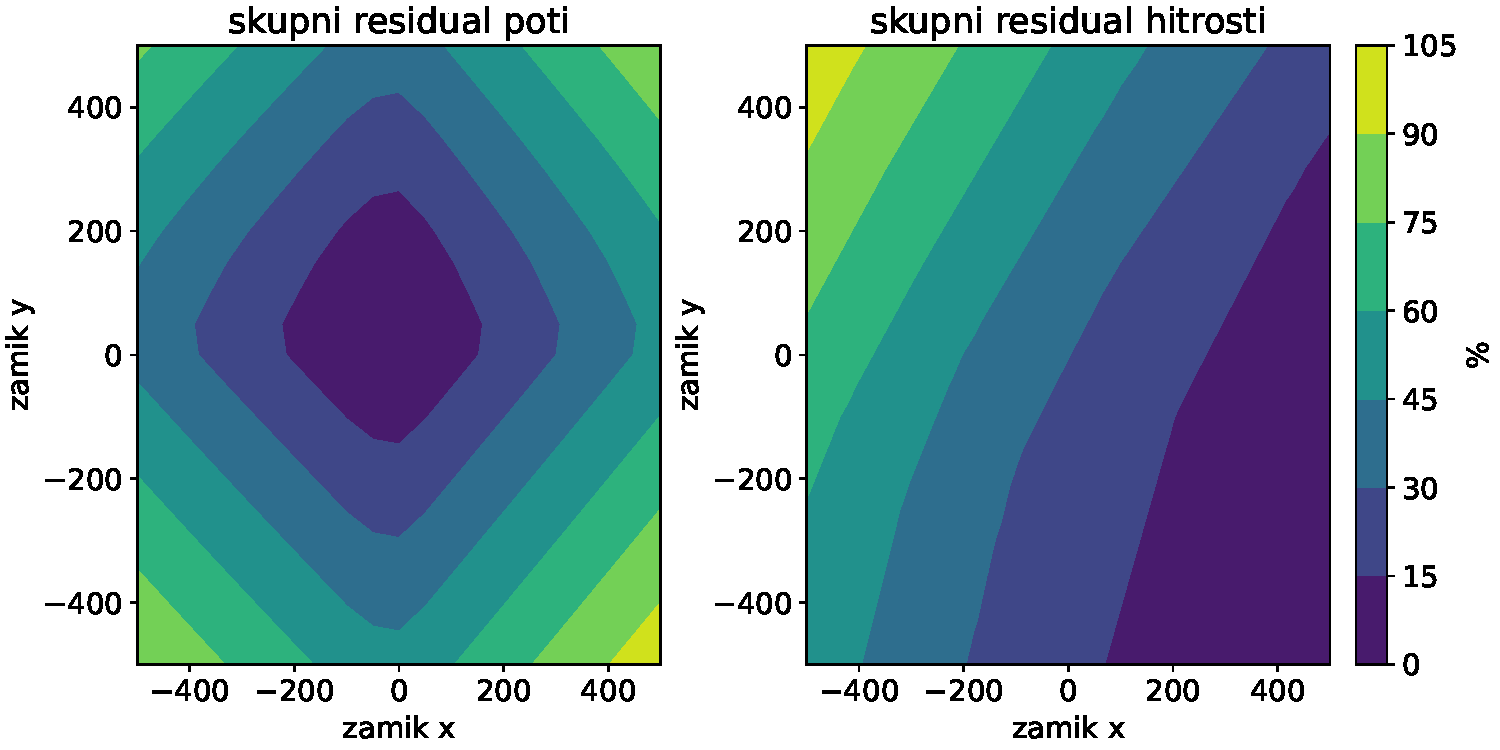
\includegraphics[width=0.65\textwidth]{11.nal_slike/vpliv_zamikov_lege.pdf}
    \caption[short]{Vpliv zamika lege na napako}
\end{figure}

\begin{figure}[H]
    \centering
    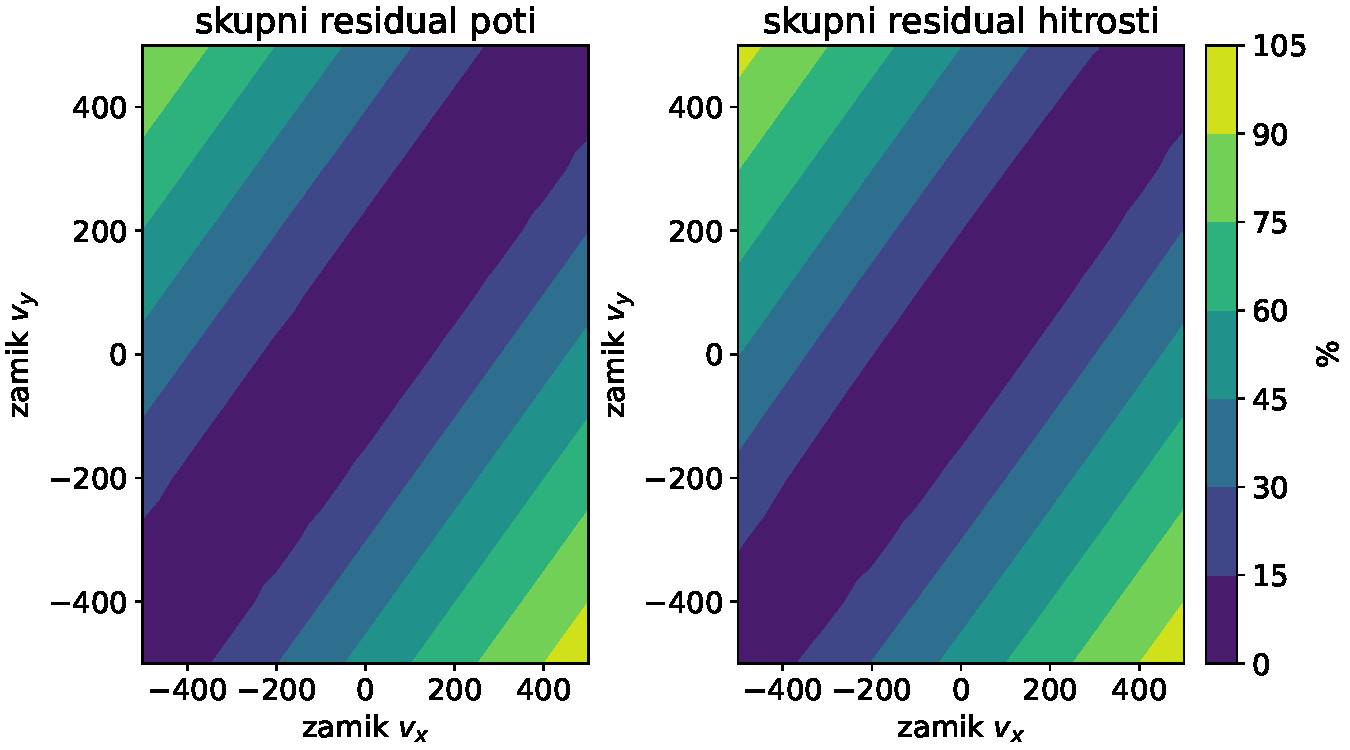
\includegraphics[width=0.65\textwidth]{11.nal_slike/vpliv_zamikov_hitrosti.pdf}
    \caption[short]{Vpliv napačne začetne hitrosti na napako}   
\end{figure}

\begin{figure}[H]
    \centering
    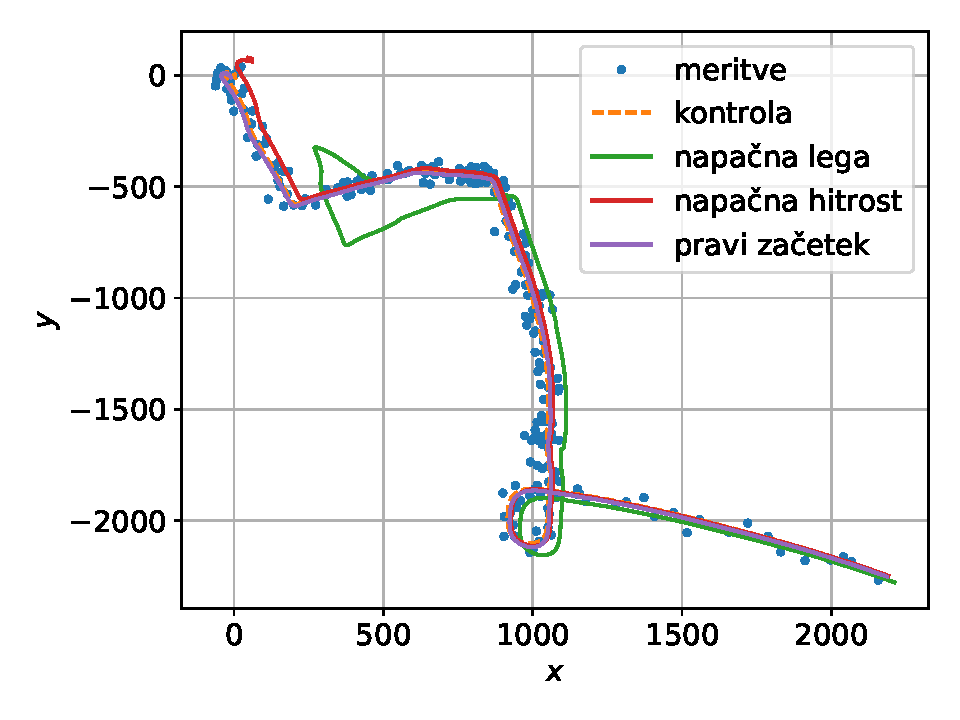
\includegraphics[width=0.5\textwidth]{11.nal_slike/pot_zamiki.pdf}
    \caption[short]{Grafični prikaz napačne lege $(x_0+500,y_0-500)$ in hitrosti $(v_{x0}+500,v_{y0}+500)$ ter primerjava z referenco}
\end{figure}

%%%%%%%%%%%%%%%%%%%%%%%%%%%%%%%%%%%%%%%%5
\section{Izpust podatkov}

    \subsection{Brez hitrosti}

Opazimo, da ob izpustu podatkov o hitrosti iz vektorja meritev -- korak je večji od števila podatkov, globalno ni opaznih sprememb, v detajlu pa vidimo kako se filter ``lovi''. Zato naraste tudi napaka, če primerjamo sliki \ref{fig:napake} in  \ref{fig:napaka_brez_v} vidimo, da smo na napaki pridobili veliko vrhov, kar nakazuje, da se filter na vsake toliko časa ``ujame'' s podatki.

\begin{figure}[H]
    \begin{minipage}{0.49\textwidth}
        \centering
        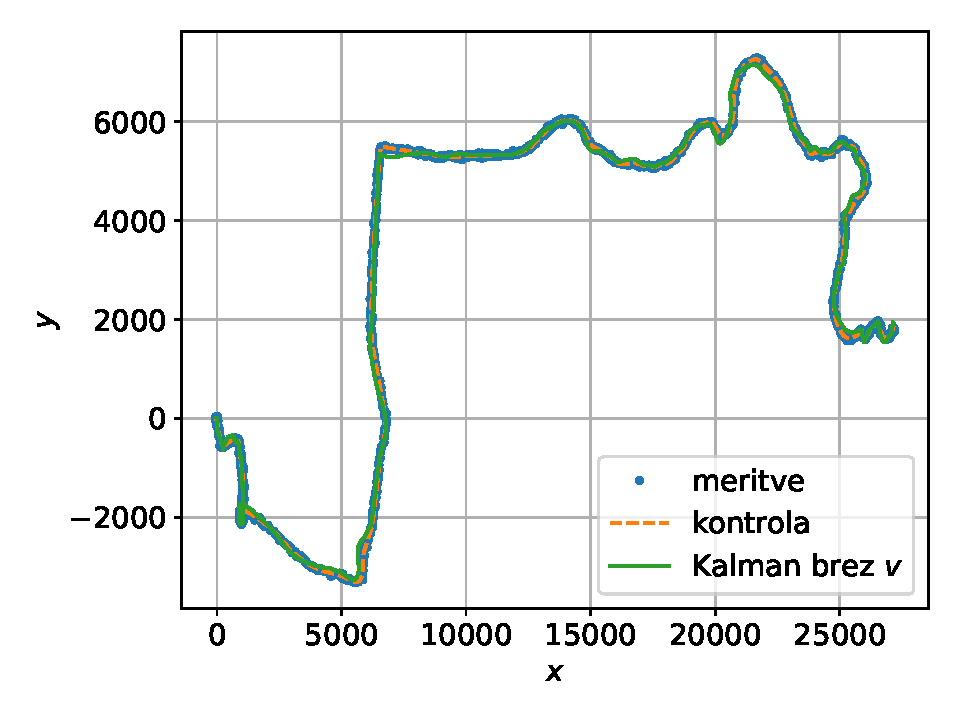
\includegraphics[width=\linewidth]{11.nal_slike/pot_brez_vdata.pdf}
        \caption[short]{Pot brez podatkov o hitrosti}
    \end{minipage}
    \begin{minipage}{0.49\textwidth}
        \centering
        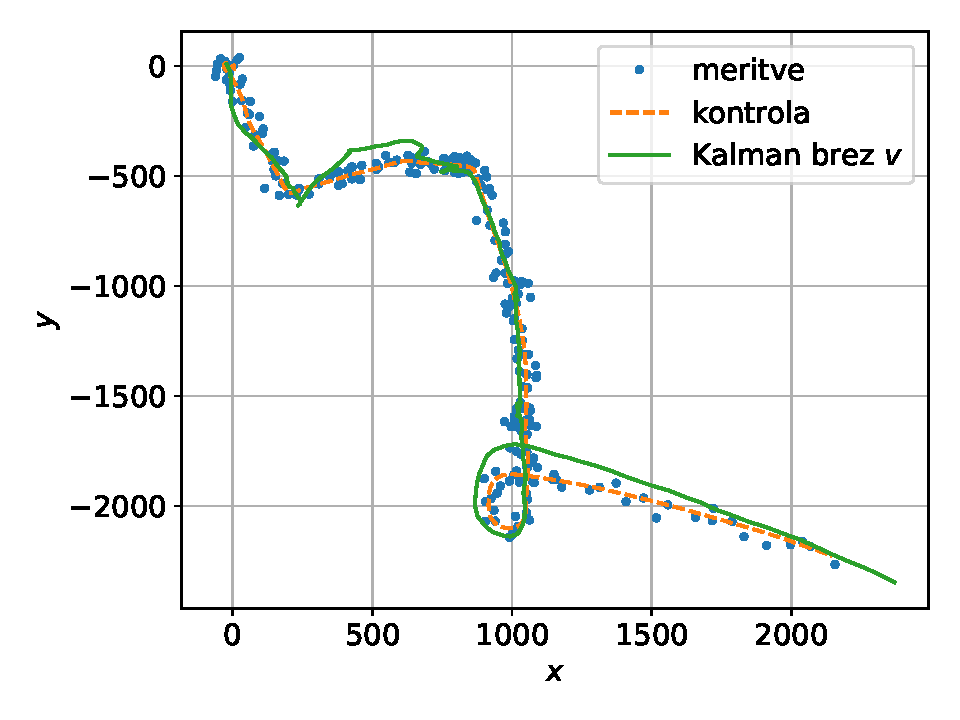
\includegraphics[width=\linewidth]{11.nal_slike/pot_brez_vdata_detajl.pdf}
        \caption[short]{detajl poti}
    \end{minipage}
\end{figure}

\begin{figure}[H]
    \centering
    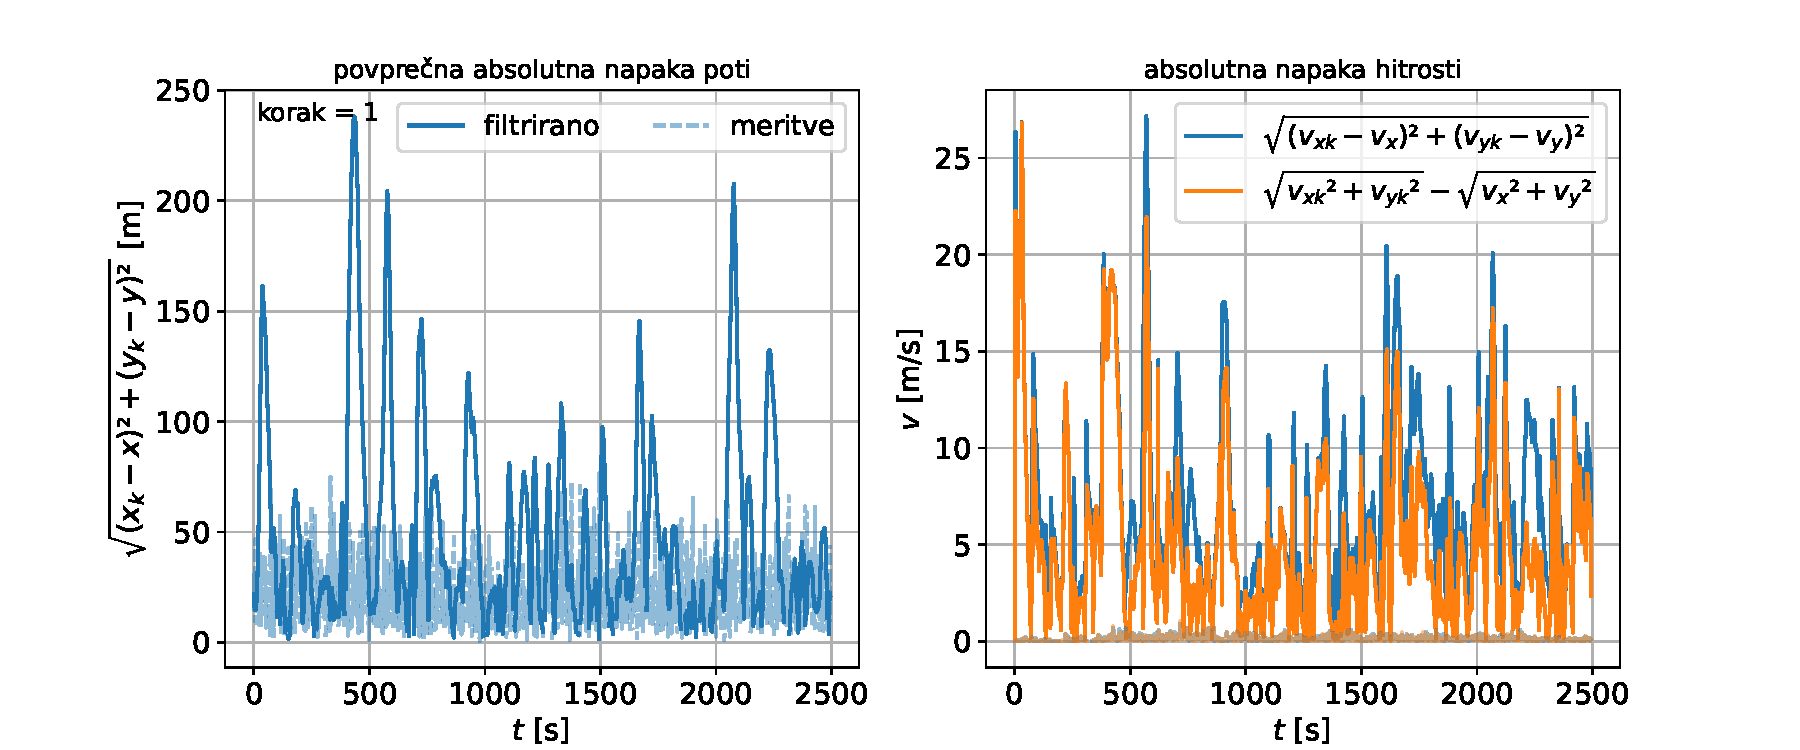
\includegraphics[width=0.9\textwidth]{11.nal_slike/napaka_poti_brez_vdata.pdf}
    \caption[short]{Potek napake pri podatkih brez hitrosti}\label{fig:napaka_brez_v}
\end{figure}

    \subsection{Brez lege}

Na enak način, kot sem izpustil podatke o hitrosti, lahko naredimo tudi z lego. Opazimo, da filter že iz hitrosti in pospeškov presenetljivo dobro ujame smer. Le po dokaj dolgih razdaljah prihaja do vidnih odstopanj. Napaka hitrosti se sicer poveča, bolj opazno pa raste napaka lege.\\
Opomba: uporabljen je korak 10 na hitrosti, da so rezultati bolj opazni. Pri uporabi vseh meritev, napaka lege na prvi sliki ne bi bila opazna.

\begin{figure}[H]
    \centering
    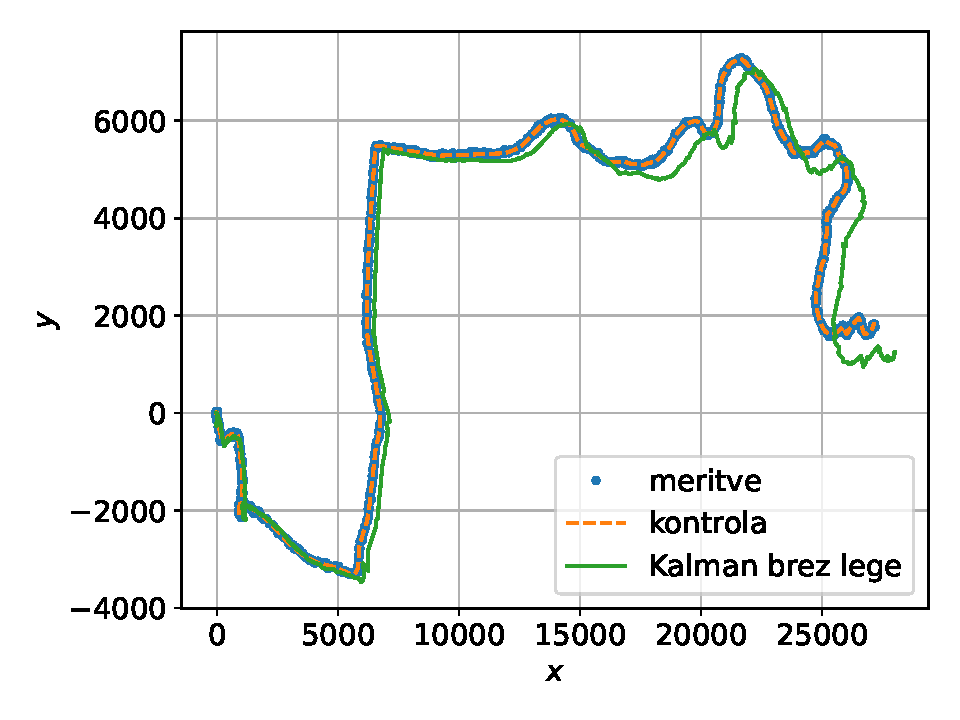
\includegraphics[width=0.5\textwidth]{11.nal_slike/pot_brez_lege.pdf}
    \caption[short]{Filtrirana pot brez podatkov o legi s korakom 10}
\end{figure}

\begin{figure}[H]
    \centering
    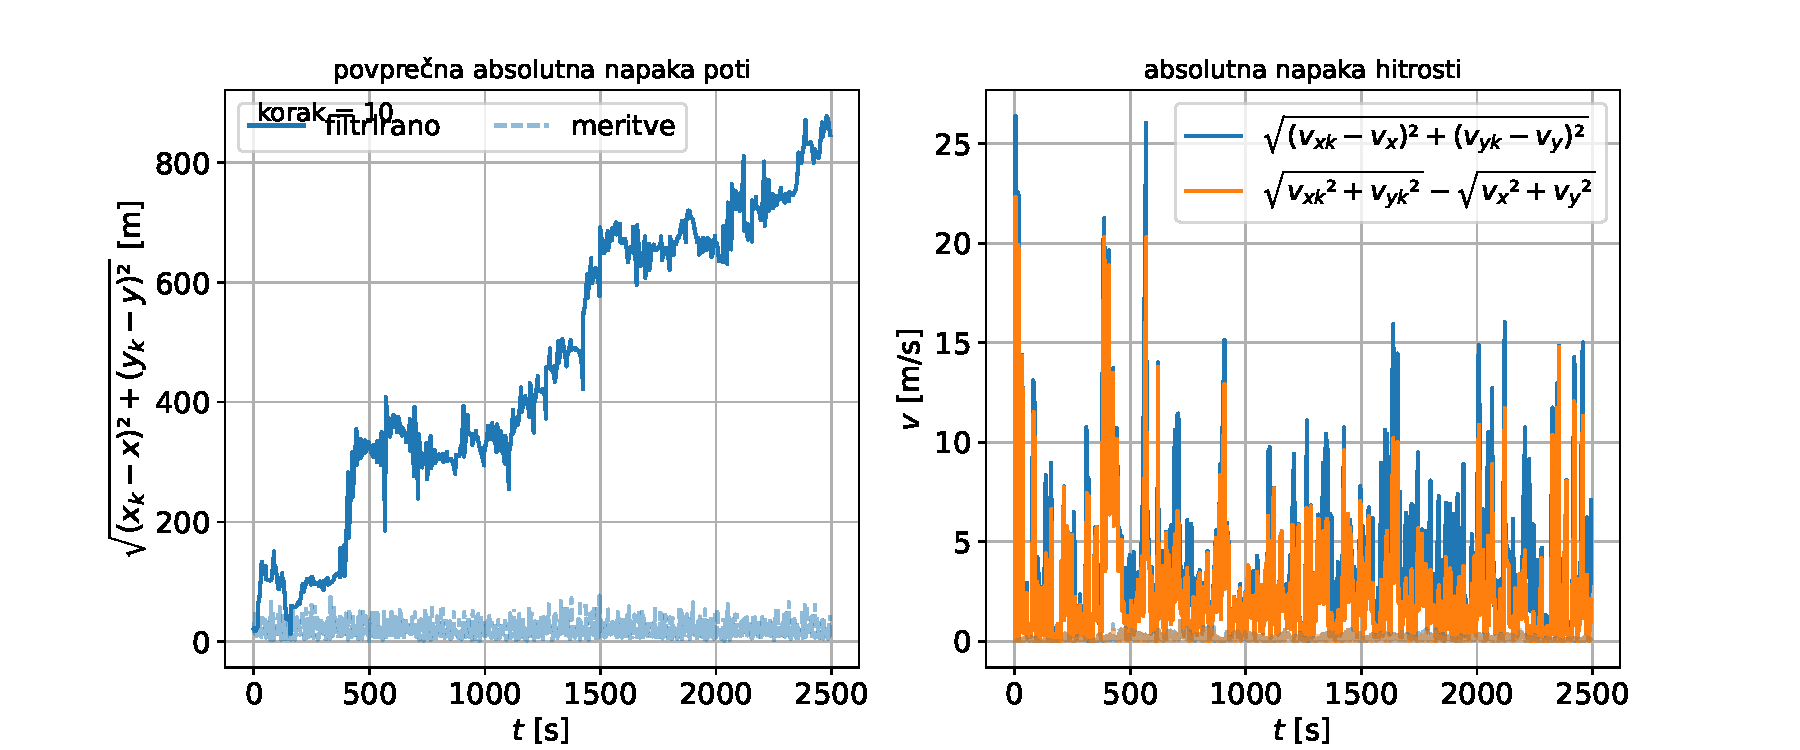
\includegraphics[width=0.9\textwidth]{11.nal_slike/napaka_poti_brez_lege.pdf}
    \caption[short]{Potek napake pri podatkih brez lege s korakom 10}
\end{figure}

\subsection{Brez pospeškov}

Lahko tudi poizkusimo in izpustimo kontrolni vektor, ki vsebuje meritve pospeškov v podkoraku predict. Tako upoštevamo le uporabljen kinematični zakon v prehodni matriki. Opazim, da to na rezultat vpliva v manjši meri.

\begin{figure}[H]
    \centering
    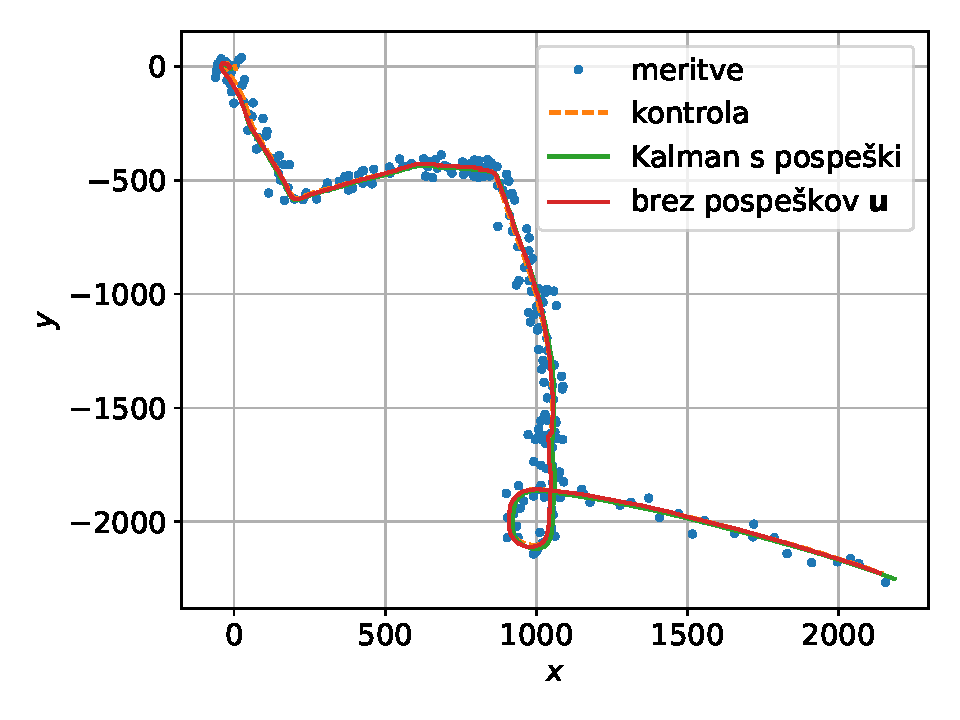
\includegraphics[width=0.5\textwidth]{11.nal_slike/pot_brez_adata_detajl.pdf}
    \caption[short]{Filtrirana pot brez podatkov o pospeških}
\end{figure}

\begin{figure}[H]
    \centering
    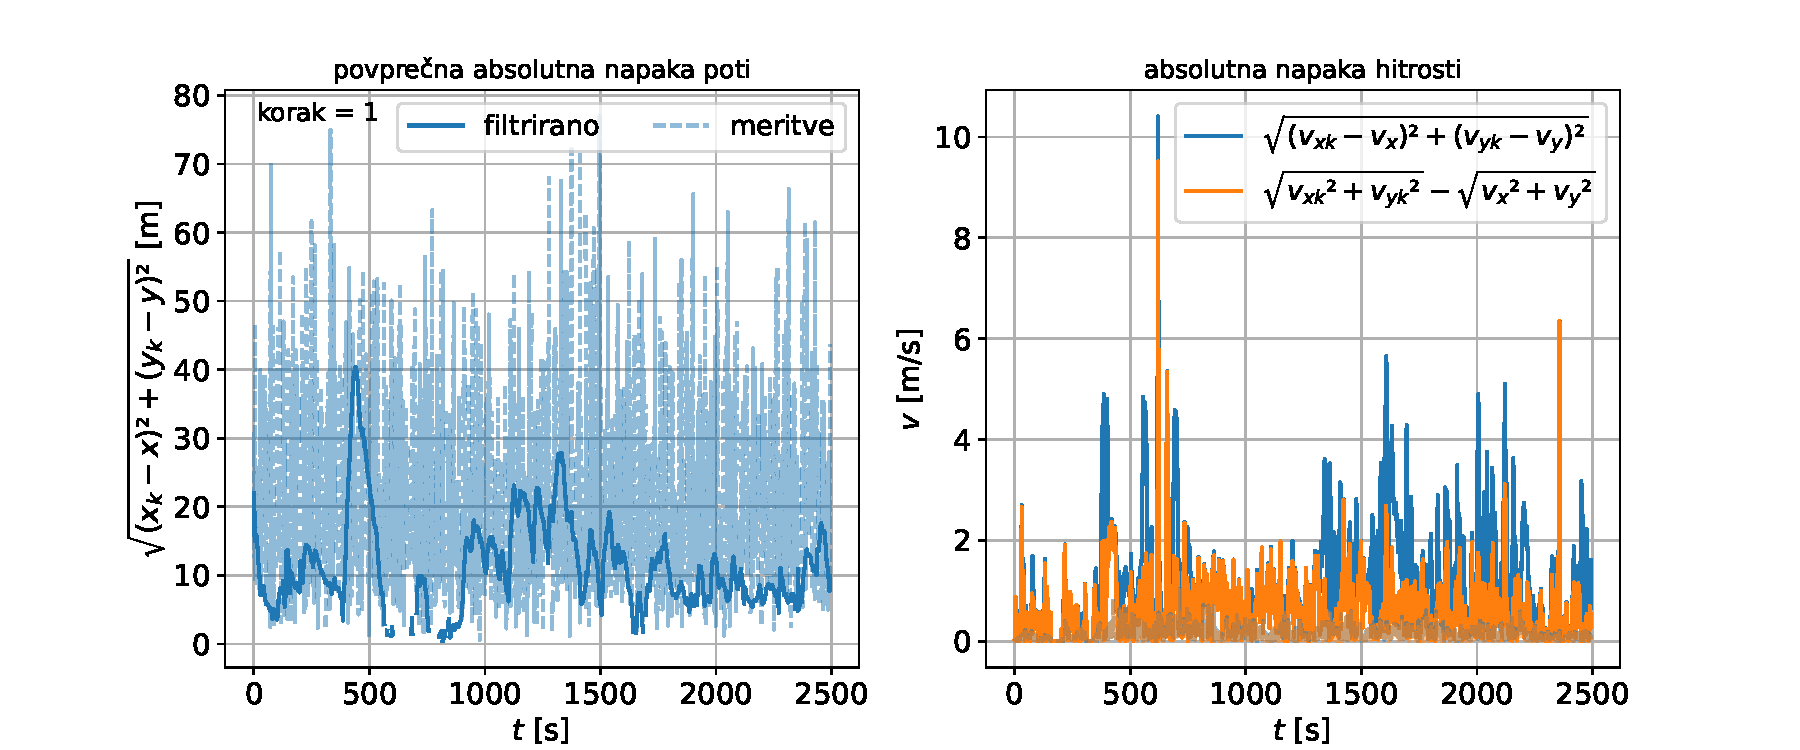
\includegraphics[width=0.9\textwidth]{11.nal_slike/napaka_poti_brez_adata.pdf}
    \caption[short]{Potek napake pri podatkih brez pospeškov}
\end{figure}

    \subsection{Le pospeški}

Če popolnoma izločimo dotok meritev v podkoraku update, filter izgubi orientacijo. Nekatere izrazite spremembe smeri se sicer vseeno izražajo, vendar je lega popolnoma napak. V detajlu je vidno, da filter lahko tako lahko deluje le na zelo kratkih razdaljah, saj se hitro izgubi. Pri tem velja podariti, kako pomembne so meritve lege!

\begin{figure}[H]
    \begin{minipage}{0.49\textwidth}
        \centering
        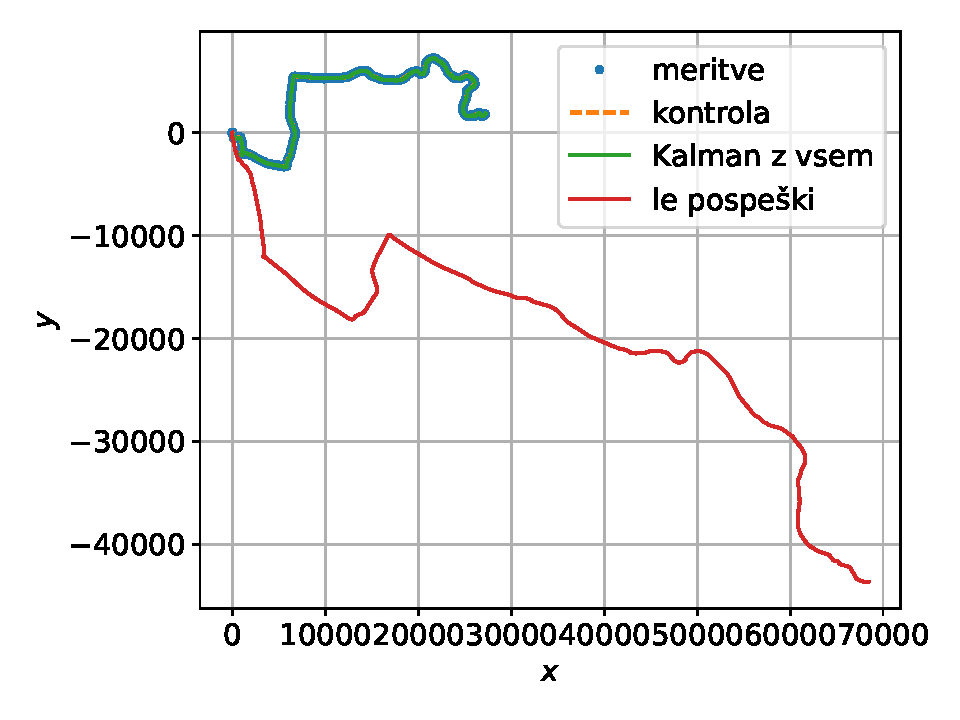
\includegraphics[width=\linewidth]{11.nal_slike/pot_le_pospeški.pdf}
        \caption[short]{Pot, ko so na voljo le pospeški}
    \end{minipage}
    \begin{minipage}{0.49\textwidth}
        \centering
        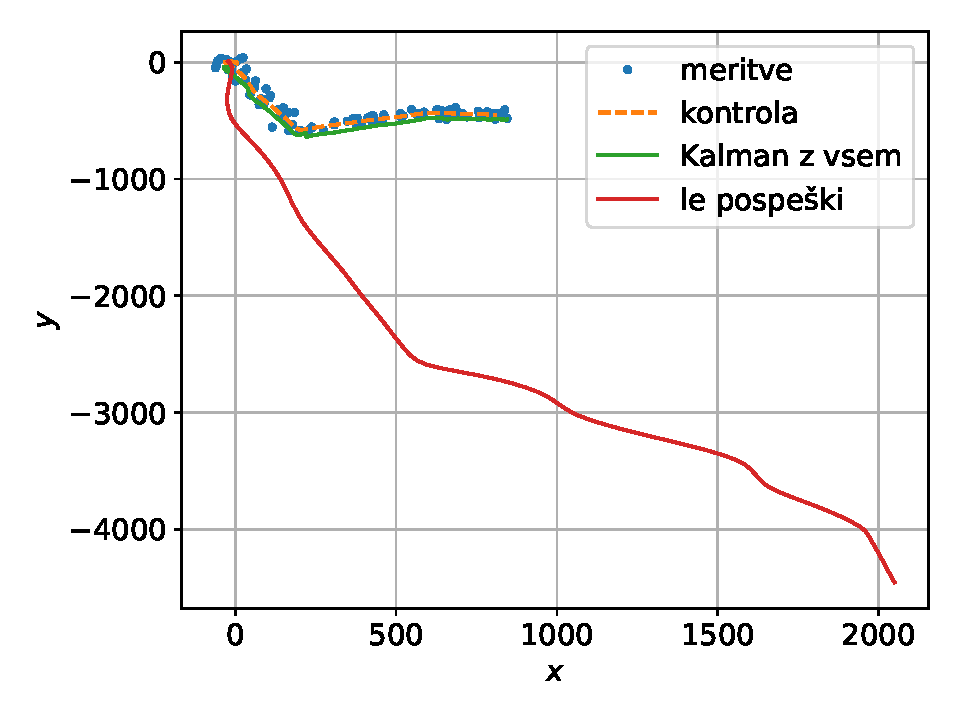
\includegraphics[width=\linewidth]{11.nal_slike/pot_le_pospeški_detajl.pdf}
        \caption[short]{detajl poti}
    \end{minipage}
\end{figure}

%     \subsection{Brez pospeškov in lege}

% \begin{figure}[H]
%     \centering
%     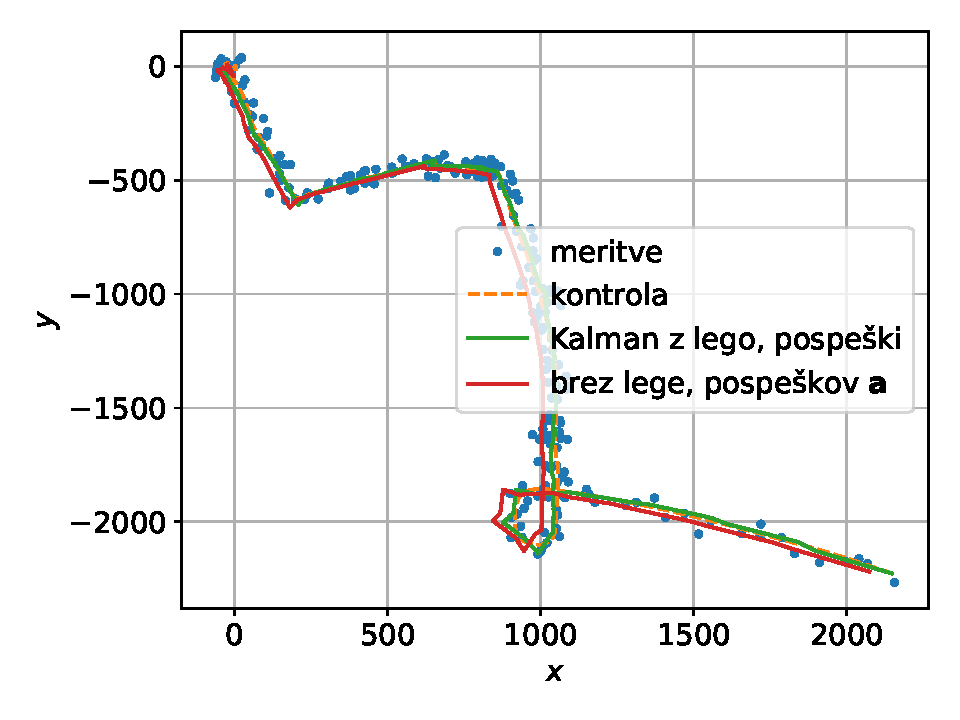
\includegraphics[width=0.5\textwidth]{11.nal_slike/pot_brez_lege_adata.pdf}
%     \caption[short]{Filtrirana pot brez podatkov o legi in pospeških s korakom 5}
% \end{figure}

%%%%%%%%%%%%%%%%%%%%%%%%%%%%%%%%%%%%%%%%%%%%%%%%%%%%%%%%%
\section{Filtriranje v naravnem koordinatnem sistemu}

Namesto v kartezičnem KS, so bili podatki podani v naravnem. Pri tem je bilo potrebno podatke o meritvah pospeškov pretvoriti v kartezični KS, lega je bila tudi podana, hitrost pa ne. Ker imamo v tem primeru na voljo le hitrost izračunano prek filtra, ki ni nikoli osvežena z meritvijo, tako dobljena hitrost bistveno odstopa od prave. Opazimo, da je na tak način filtrirana lega razmeroma ustrezna, v detajlu sicer vidimo, da se filter ne obnaša tako, kot bi želeli, globalno pa je pot ustrezna, le na nekaterih ovinkih filter malenkost ``iztiri''. Tako dobljene napake so tudi očitno višje, vendar so značilni vrhovi/doline na enakih legah (ob enakih časih).

\begin{figure}[H]
    \begin{minipage}{0.49\textwidth}
        \centering
        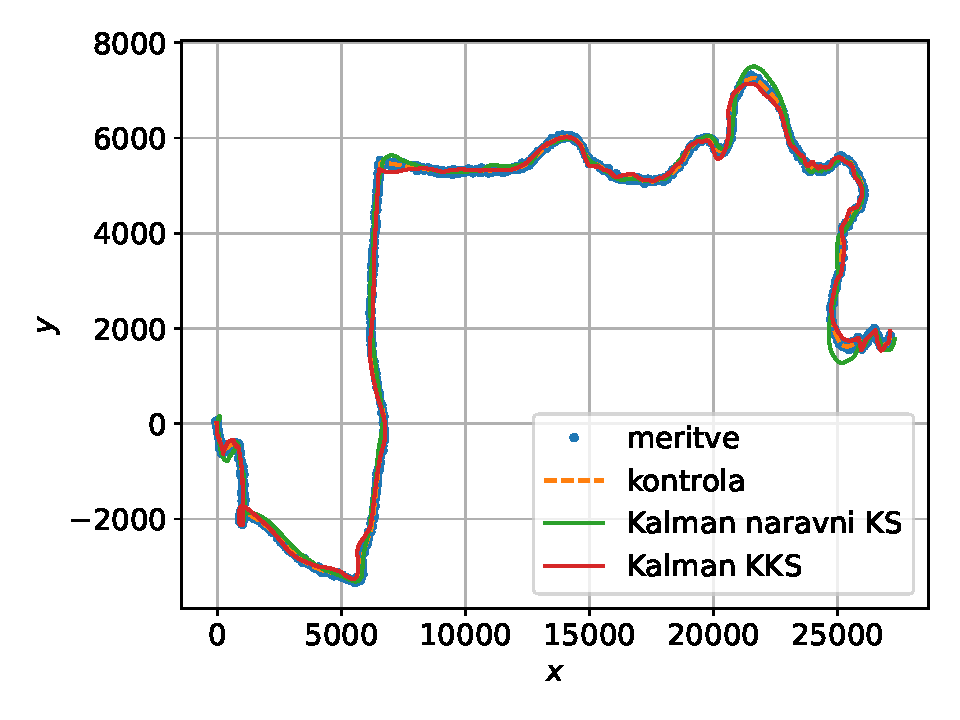
\includegraphics[width=\linewidth]{11.nal_slike/pot_relat.pdf}
        \caption[short]{Pot pri uporabi naravnega KS}
    \end{minipage}
    \begin{minipage}{0.49\textwidth}
        \centering
        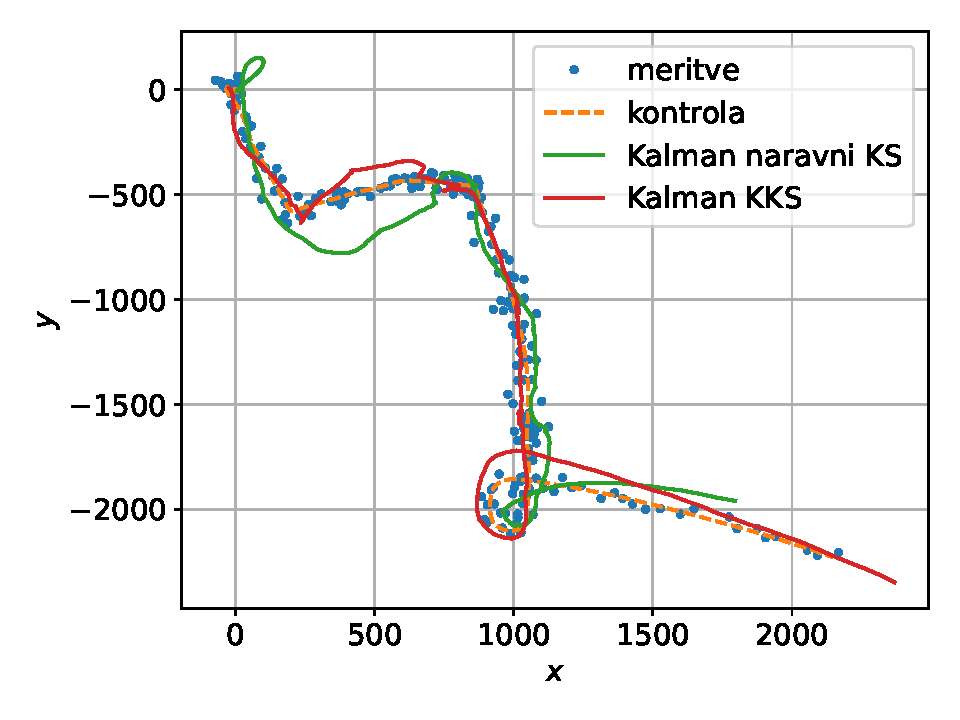
\includegraphics[width=\linewidth]{11.nal_slike/pot_relat_detajl.pdf}
        \caption[short]{detajl poti}
    \end{minipage}
\end{figure}

\begin{figure}[H]
    \centering
    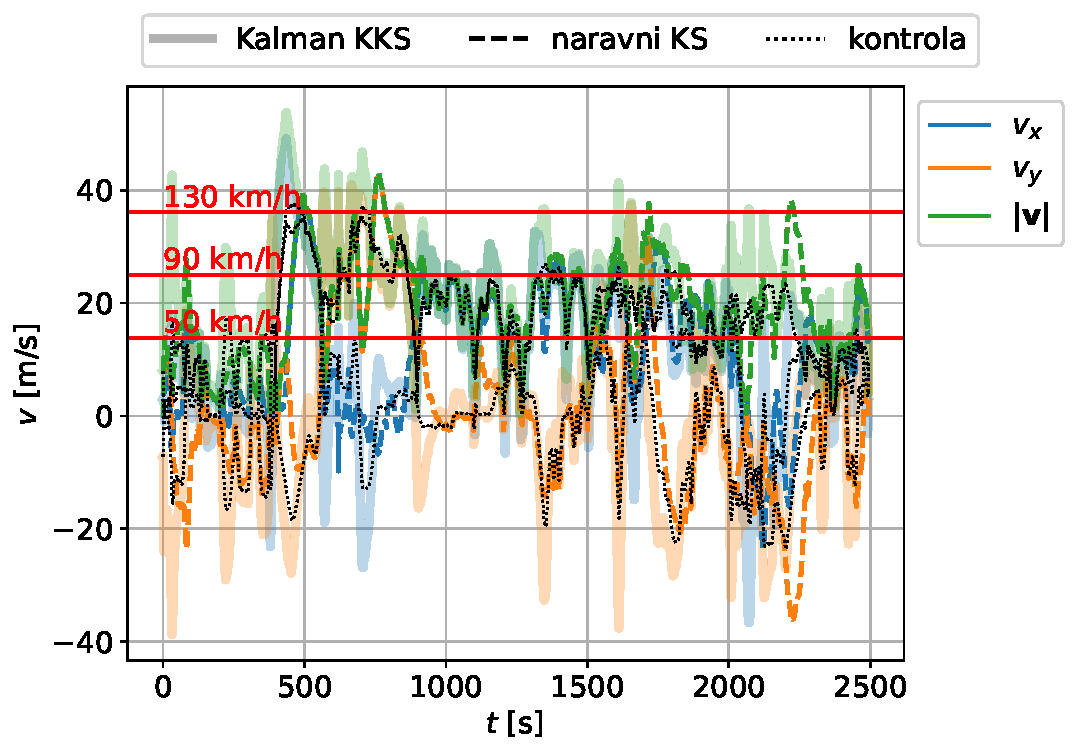
\includegraphics[width=0.5\textwidth]{11.nal_slike/potek_hitrosti_relat.pdf}
    \caption[short]{Potek izračunanih hitrosti v naravnem KS}
\end{figure}

\begin{figure}[H]
    \centering
    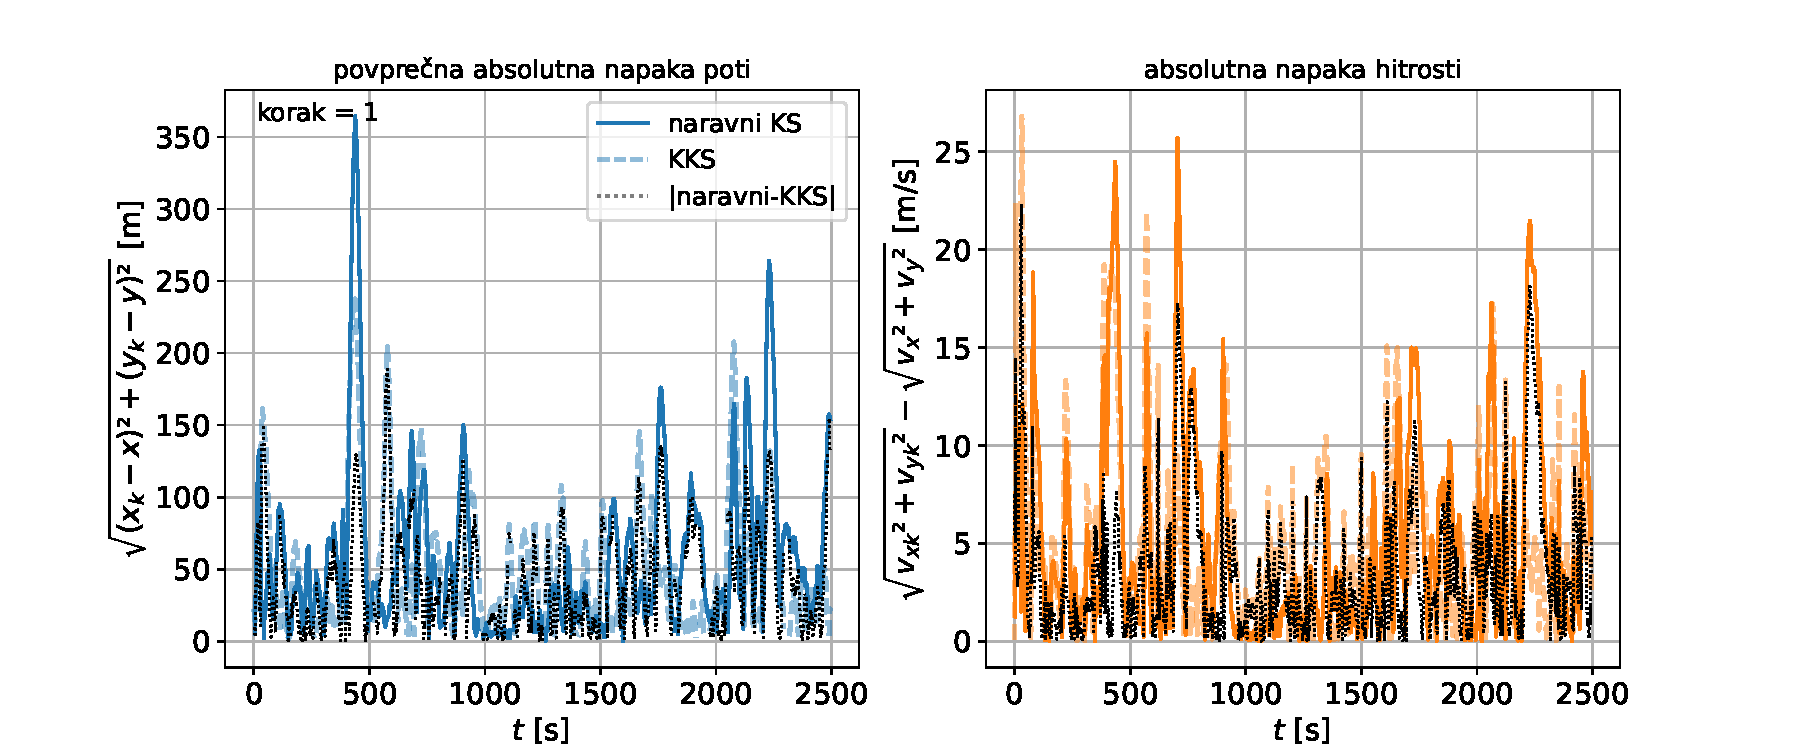
\includegraphics[width=0.9\textwidth]{11.nal_slike/napaka_poti_hitrosti_relat.pdf}
    \caption[short]{Potek napake pri podatkih v naravnem KS}
\end{figure}

Če primerjam še skupni residual za različne korake, tega ne morem prikazati barvnem grafu, kot poprej, saj je tukaj na voljo le en korak (za podatke lege). V bolj preprosti obliki vidimo podoben trend naraščanja z večanjem koraka, to mopeni večje število izpuščenih podatkov.

\begin{figure}[H]
    \centering
    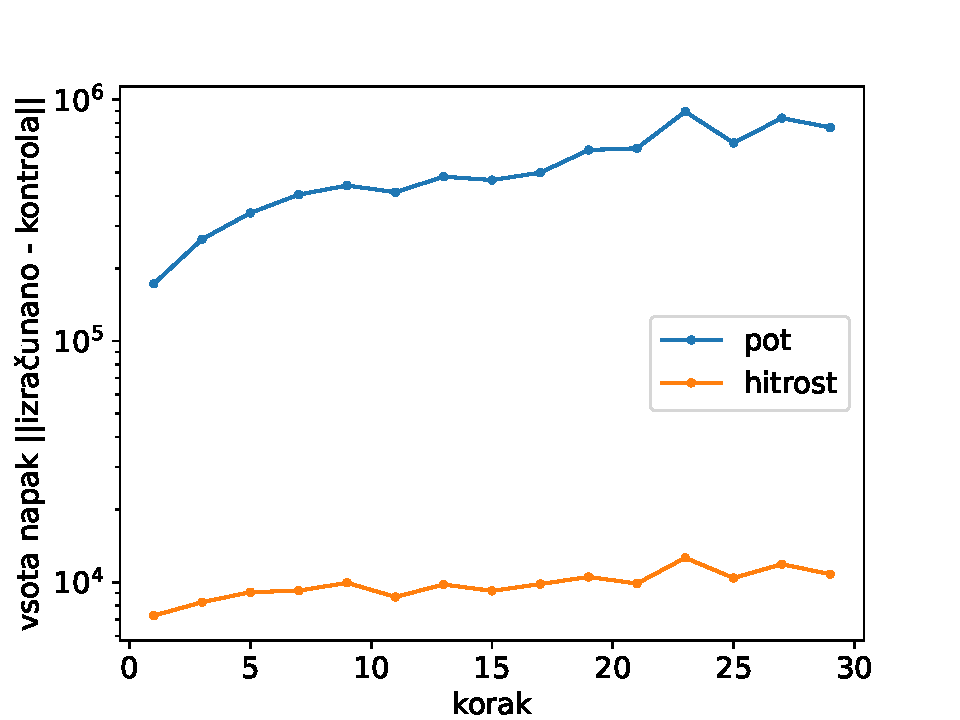
\includegraphics[width=0.6\textwidth]{11.nal_slike/napaka_koraki_naravni.pdf}
    \caption[short]{Vpliv koraka pri uporabi podatkov na napako poti in hitrosti}
\end{figure}

%%%%%%%%%%%%%%%%%%%%%%%%%%%%%%
\section{Podatki v 3D - letenje}

Ker imam na voljo še podatke s testiranja modelarskega letala, sem poskusil filtrirati še te. Podatki o legi so namreč bili težko berljivi. Kmalu sem ugotovil, da je to težka naloga, saj sem imel na voljo le sledeče podatke:\\
čas, koordinate, višino, ground speed, air speed, moč motorja, el. tok, napetost baterije\dots

Ker je bilo takorekoč skoraj nič uporabnih izmerjenih podatkov, sem po težavah s singularnimi matrikami v filtru nalogo opustil, čeprav bi bilo mogoče iz absolutne (ground speed) hitrosti in trajektorije določiti komponente hitrosti. Tukaj predstavljam zgolj surove podatke za en krog letenja.

\begin{figure}[ht!]
    \centering
    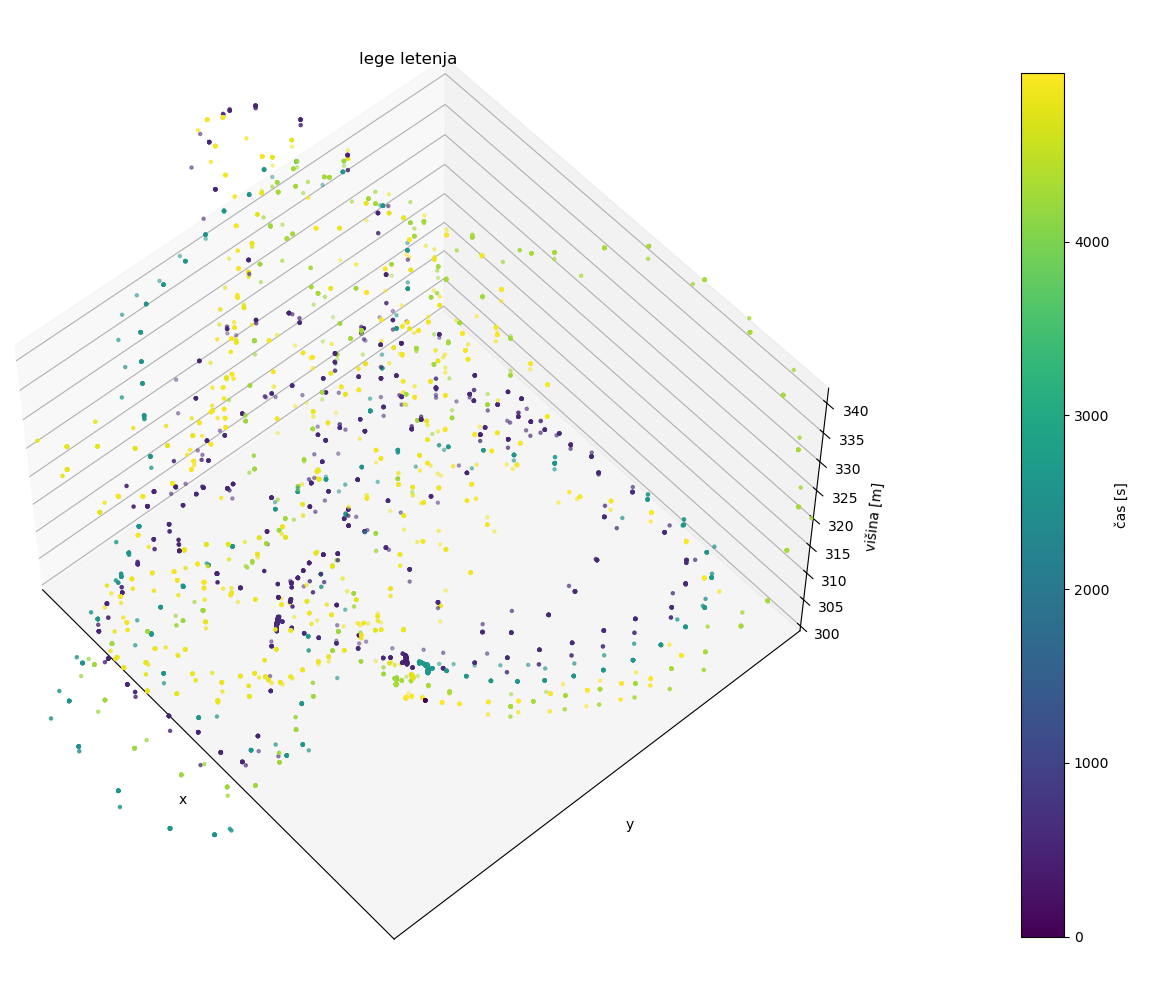
\includegraphics[width=\textwidth]{11.nal_slike/letalo.png}
    \caption[short]{GPS točke letenja}
\end{figure}

\begin{figure}[ht!]
    \centering
    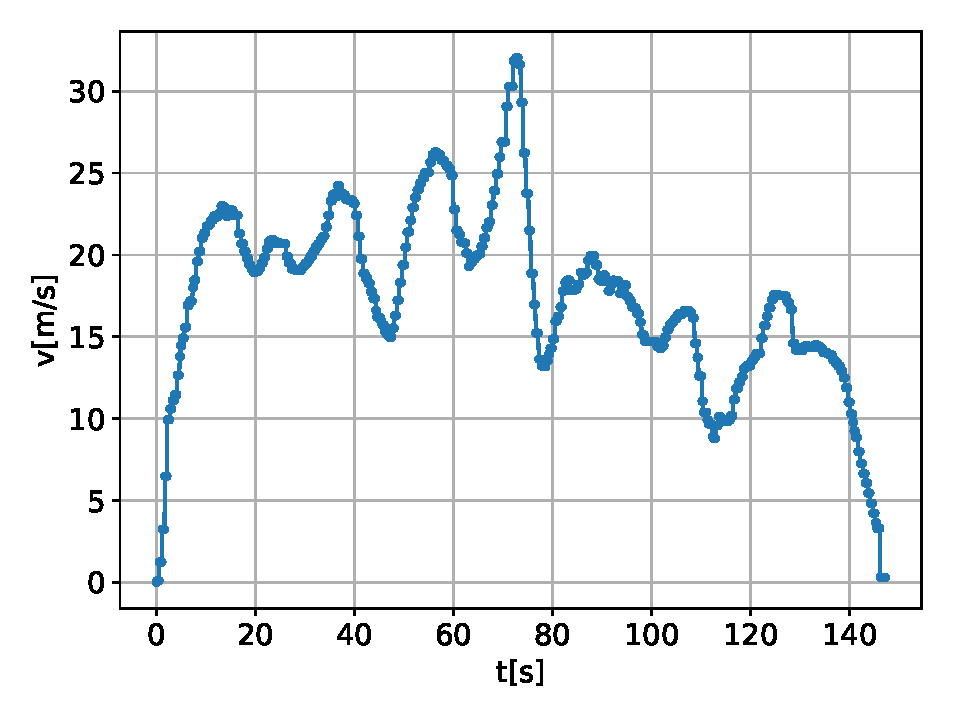
\includegraphics[width=0.5\textwidth]{11.nal_slike/3d_hitrosti_krog.pdf}
    \caption[short]{Potek hitrosti}
\end{figure}